\section{Performance Modeling}
\label{sec:performance-modeling}

The first step towards bounded response times is to model the relationship
between accuracy and execution time. We then describe the formalism and our
data-driven approach.

\subsection{Problem Formulation}
\label{sec:problem-formulation}

We assume there are multiple algorithms $\mathbb{A}$ available to provide the
same inference. For each algorithm $a \in \mathbb{A}$, it has parameters tunable
to affect processing time $t$ and inference accuracy (or utility $u$). These
parameters could be related to data, such as lowering the image resolution, or
related to the algorithm, such as increasing the scaling factor in HOG. One
instance of the parameters forms a configuration
$\vec{c} = (k_1, k_2, \dots, k_n)$ with $n$ dimensions---we explicitly use the
arrow head here to emphasize configurations' high dimensionality. Running the
algorithm $a$ with a configuration $\vec{c}$ on a machine $m$ yields an
inference with utility $u$ and processing time $t$.

We denote this performance model as a mapping:

{\small \vspace{-1em}
  \begin{equation*}
    f: (\mathbb{A} \times \mathbb{P} \times \mathbb{M}) \rightarrow
    (\mathbb{R}\times \mathbb{R})
\end{equation*}
} where $\mathbb{A}$ is the set of all algorithms, $\mathbb{C}$ is the set of
all possible configurations, and $\mathbb{M}$ is the set of all machines. The
mapping returns two real values: execution time $t \in \mathbb{R}$ and utility
$u \in \mathbb{R}$. For convenience, we use $\vec{x}$ for the tuple $(a, c, m)$.
Also we use $f_t$ and $f_u$ for the mapping from variables to time $t$ and
utility $u$, respectively.

Bounding the response times is trivial if application accuracy can be
arbitrarily low. \sysname{} aims to minimize response times while maximizing
achievable accuracy---solving a multi-objective optimization problem,
specifically two objectives. For these problems in general, there is no single
optimal solution that jointly minimizes multiple objectives. Instead, there is a
collection of optimal solutions where for any solution, no objective can be
improved without damaging one of the other objectives. The goal of our
performance modeling is to derive such Pareto-optimal
set~\cite{collette2013multiobjective} across all possible
configurations. Formally, the Pareto-optimal set is defined as follows,

{\small \vspace{-1.2em}
  \begin{equation}
    \mathbb{P} = \{ \vec{x} \in \mathbb{X} : \{ \vec{x'} \in \mathbb{X}:
    f_t(\vec{x'}) < f_t(\vec{x}), f_u(\vec{x'}) > f_u(\vec{x}) \} = \varnothing\}
  \label{eq:pareto}
\end{equation}
\vspace{-1.2em}
}

\para{Challenge.} The Pareto-optimal set is easy if we know the mapping for all
possible arguments. However, in practice, the argument space is prohibitively
large, especially for configurations $\vec{c}$ that have many tunable
parameters. It is expensive to run all combinations. Besides, it is also
impossible because developers may not have target machines available.

\para{Solution Overview.} We tackle each dimension differently. For algorithms,
because their differences are substantial, our profiler evaluates all available
algorithms exhaustively. For each algorithm, to address the curse of
dimensionality of $\vec{c}$, we use BO to reduce space search and only find
near-optimal $c$s. For different machine $m$, because only $f_t$ depends on $p$,
we show that the Pareto-optimal set doesn't change if the execution time $f_t$
satisfies monotonicity. We approximate $f_t$ with a simple linear model.

\subsection{Composing Algorithms}
\label{sec:compose-models}

There are different algorithms. Different implementation for GPU and CPU.

We have to profile each individual algorithm.

Observation: their profile (the Pareto-optimal set) are composable by merge and
compare all of them.

\subsection{Modeling Parameters}
\label{sec:single-platform}

\subsection{Bayesian Optimization}
\label{sec:bo}

Bayesian optimization approximate black-box functions with proxy functions and
iteratively proposes new sample point in the large parameter space. Effective
for,

\begin{itemize}
\item Evaluating each sample is expensive.
\item The objective is a black-box.
\item The evaluation can be noisy
\end{itemize}

Gaining attraction beyond ML scope:

\begin{itemize}
\item CherryPick~\cite{alipourfard2017cherrypick} finds the best cloud
  configurations for big data analytics.
\item Google optimize chocolate chip cookies recipes~\cite{solnik2017bayesian}.
\end{itemize}

\begin{figure}
  \begin{subfigure}{0.55\textwidth}
    \centering
    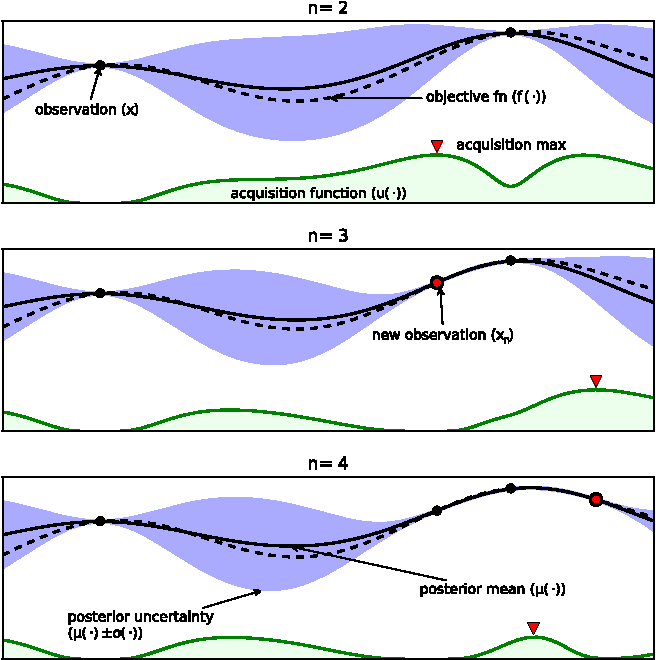
\includegraphics[width=0.8\textwidth]{figures/serving-bo-illustration.pdf}
    \caption{Acquisition function evaluates the utility of candidate points for
      the next evaluation of $f$, balancing a high objective (exploitation) and
      high uncertainty (exploration)~\cite{shahriari2016taking}.}
  \end{subfigure}%
  \hfill
  \begin{subfigure}{0.35\textwidth}
    \centering
    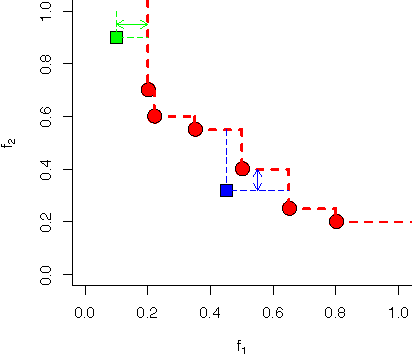
\includegraphics[width=0.8\textwidth]{figures/serving-bo-2d-1.pdf} \\
    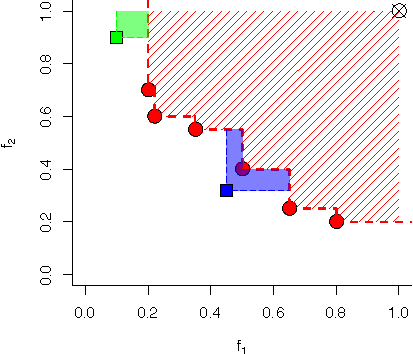
\includegraphics[width=0.8\textwidth]{figures/serving-bo-2d-2.pdf}
    \caption{For two-objective optimization, utility gain is based on
      additive-epsilon (top) or hypervolume (bottom)~\cite{binoisgpareto}.}
  \end{subfigure}
\end{figure}


We use PESMO~\cite{hernandez2016predictive} and compare it with two baselines:
(1) greedy/coordinate search; (2) random search. PESMO chooses evaluation points
to maximally reduce the entropy of the posterior distribution over the Pareto
set.

%%% Local Variables:
%%% mode: latex
%%% TeX-master: "../compute"
%%% End:


Evaluating all configurations across the large parameter space is prohibitively
expensive. To reduce the number of samples we need, \sysname{} builds a
performance model that is just accurate enough to allow us to distinguish
near-optimal configurations from the rest. This is similar to recent systems,
such as CherryPick~\cite{alipourfard2017cherrypick} and
BOAT~\cite{dalibard2017boat}, that use Bayesian optimization (BO) to improve
performance across a large number of configurations.

While previous approaches often transform the multi-objective problem into a
single-objective problem using scalarization techniques (an approach that is
expected to be suboptimal~\cite{knowles2006parego}.) We adopted the
PESMO~\cite{hernandez2016predictive}, which does not transform the
multi-objective problem into a single-objective. PESMO also has a low
computational cost. It grows linearly with respective to the total number of
objectives $K$.

\subsection{Modeling Machines}
\label{sec:performance-transfer}

We make the observation that $f_u(a, c, m)$ doesn't depend on $m$. If we assume
a monitonicity between $f_t(m_1)$ and $f_t(m_2)$, we can prove that the
Pareto-set is directly transferable. The monitonicity is a condition that if on
one platform it takes longer for one configuration,
i.e.\,$f_t(a, \vec{c}, m_1) < f_t(a, \vec{c'}, m_1)$, then it will take longer
on another platform, i.e.\,$f_t(a, \vec{c}, m_2) < f_t(a, \vec{c'}, m_2)$.

Based on these two assumption, one can prove that if $\vec{x}_i$ is in the
Pareto-optimal set $\mathbb{P}_1$ for platform $p_1$, then $\vec{x}_i$ will also
be in the Pareto-optimal set $\mathbb{P}_2$. And the profile on $p_2$ will be a
stretched or shrunk version for $p_1$ along the time dimension.

This simplifies our model transfer across platforms and makes it possible to
derive the performance model at runtime by sampling only a few performance
measures. In practice, a simple linear transformation suffices in giving a
reasonably precise transfer.
